\begin{frame}{RRC Laboratory}
  Instrumentation development at UIC's Research Resources Center --- East
  \begin{center}
    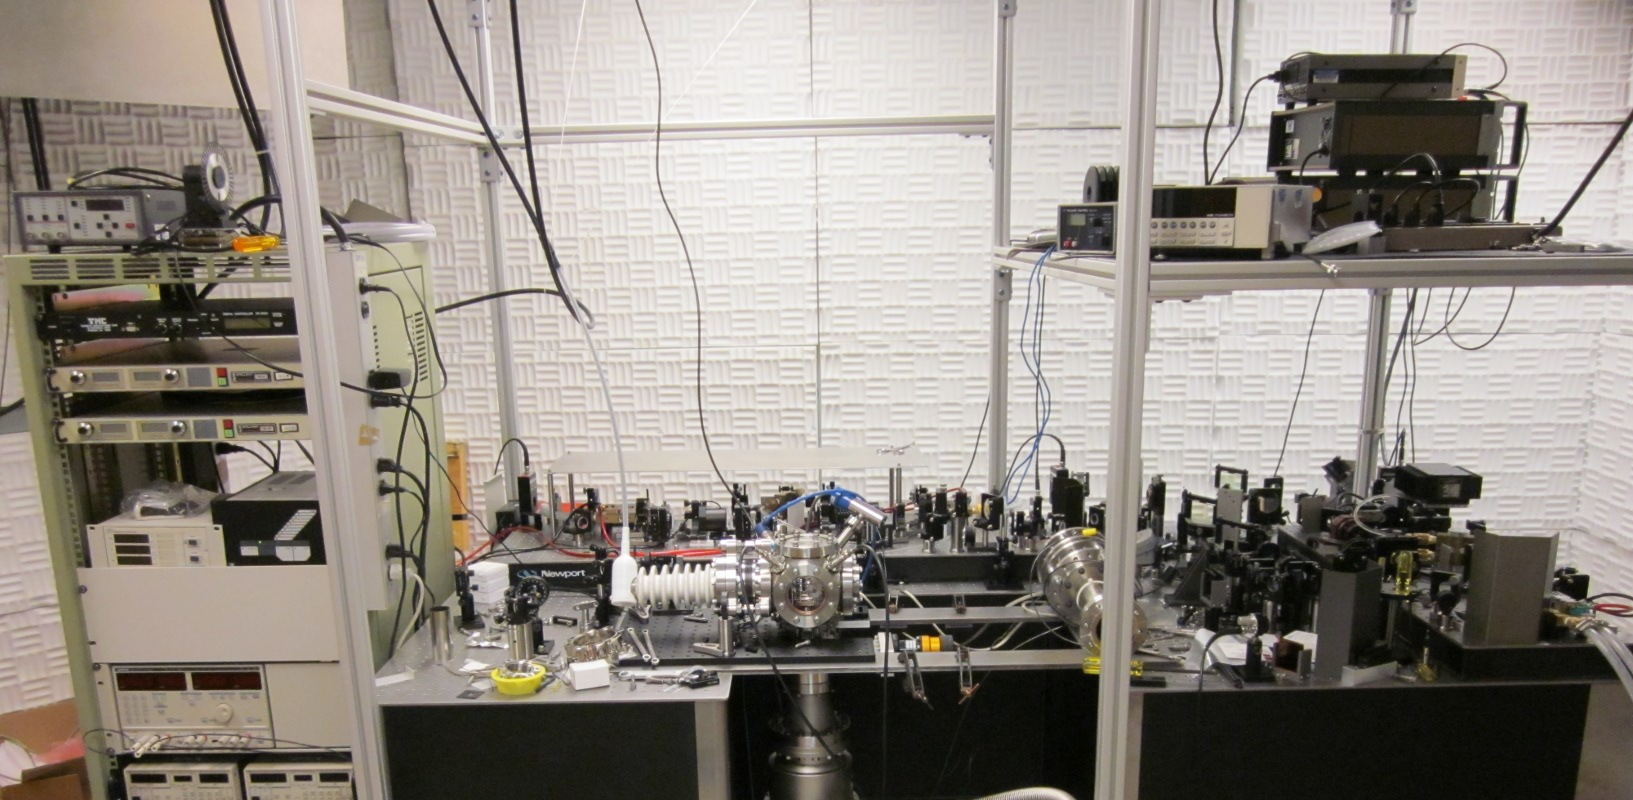
\includegraphics{lab}
  \end{center}
\end{frame}

\begin{frame}{Togawa Accelerator Design}
  The Togawa accelerator\footcite{togawa_ceb6_2007} provides
  \begin{columns}
    \begin{column}{0.49\linewidth}
      \begin{itemize}
        \item<2-> Large aperture
        \item<3-> Relatively flat electric field
        \item<4-> Low divergence near anode aperture
      \end{itemize}
      \begin{figure}
        \centering
        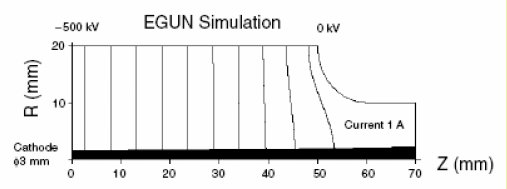
\includegraphics[width=0.9\linewidth]{Togawa_Plot}
      \end{figure}
    \end{column}
    \begin{column}{0.49\linewidth}
      \begin{itemize}
        \item<5-> Large laser angular acceptance
        \item<5-> Large photocathode area (Wehnelt)
        \item<5-> Smooth easily polished surfaces
      \end{itemize}
      \begin{figure}
        \centering
        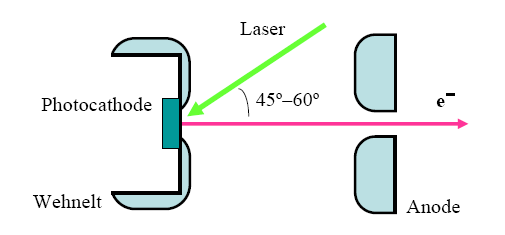
\includegraphics[width=0.9\linewidth]{Togawa}
      \end{figure}
    \end{column}
  \end{columns}
\end{frame}

\begin{frame}{Hardware Development}
  \begin{columns}
    \begin{column}{0.49\linewidth}
      Togawa Wehnelt / Anode
      \begin{figure}
        \centering
        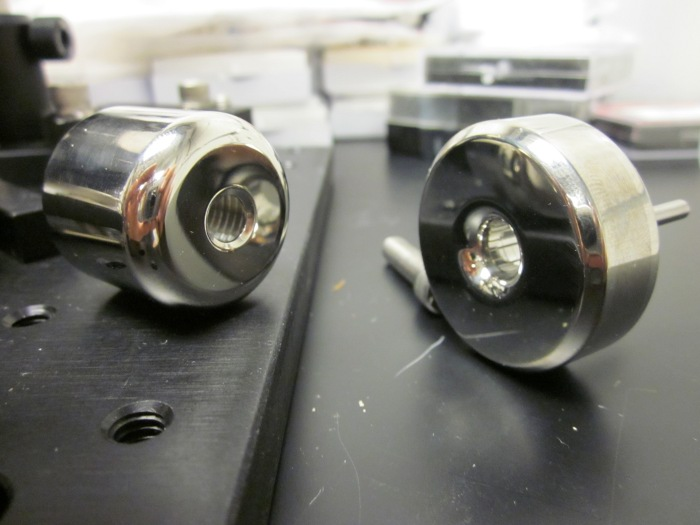
\includegraphics{anode_cathode}
      \end{figure}
    \end{column}
    \begin{column}{0.49\linewidth}
      Custom deflection plates
      \begin{figure}
        \centering
        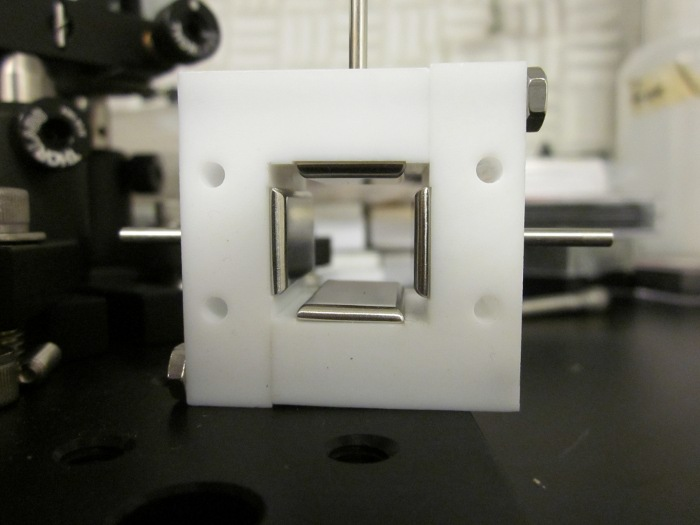
\includegraphics{deflector}
      \end{figure}
    \end{column}
  \end{columns}
  \begin{figure}
    \centering
    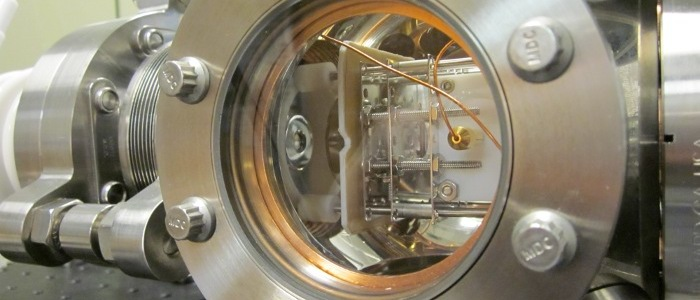
\includegraphics{chamber}
  \end{figure}
\end{frame}

\begin{frame}{Magnetic Lenses}
  For both imaging our photocathode emission and its momentum distribution (Fourier plane)
  \begin{itemize}
    \item<2-> Custom design\footcite{el-kareh_electron_1970}
    \item<3-> Large bore (aperture)
    \item<4-> High permeability pole piece (NiFe alloy $\mu \approx $50000)
  \end{itemize}
  \uncover<5->{As a pair, will be used to correct for RF cavity's inherent divergence}
\end{frame}

\begin{frame}{Magnetic Lenses Installed}
  \begin{figure}
    \centering
    \begin{tikzpicture}
      [every pin edge/.style={white,thick}]
      \begin{pgfonlayer}{background}
        \node {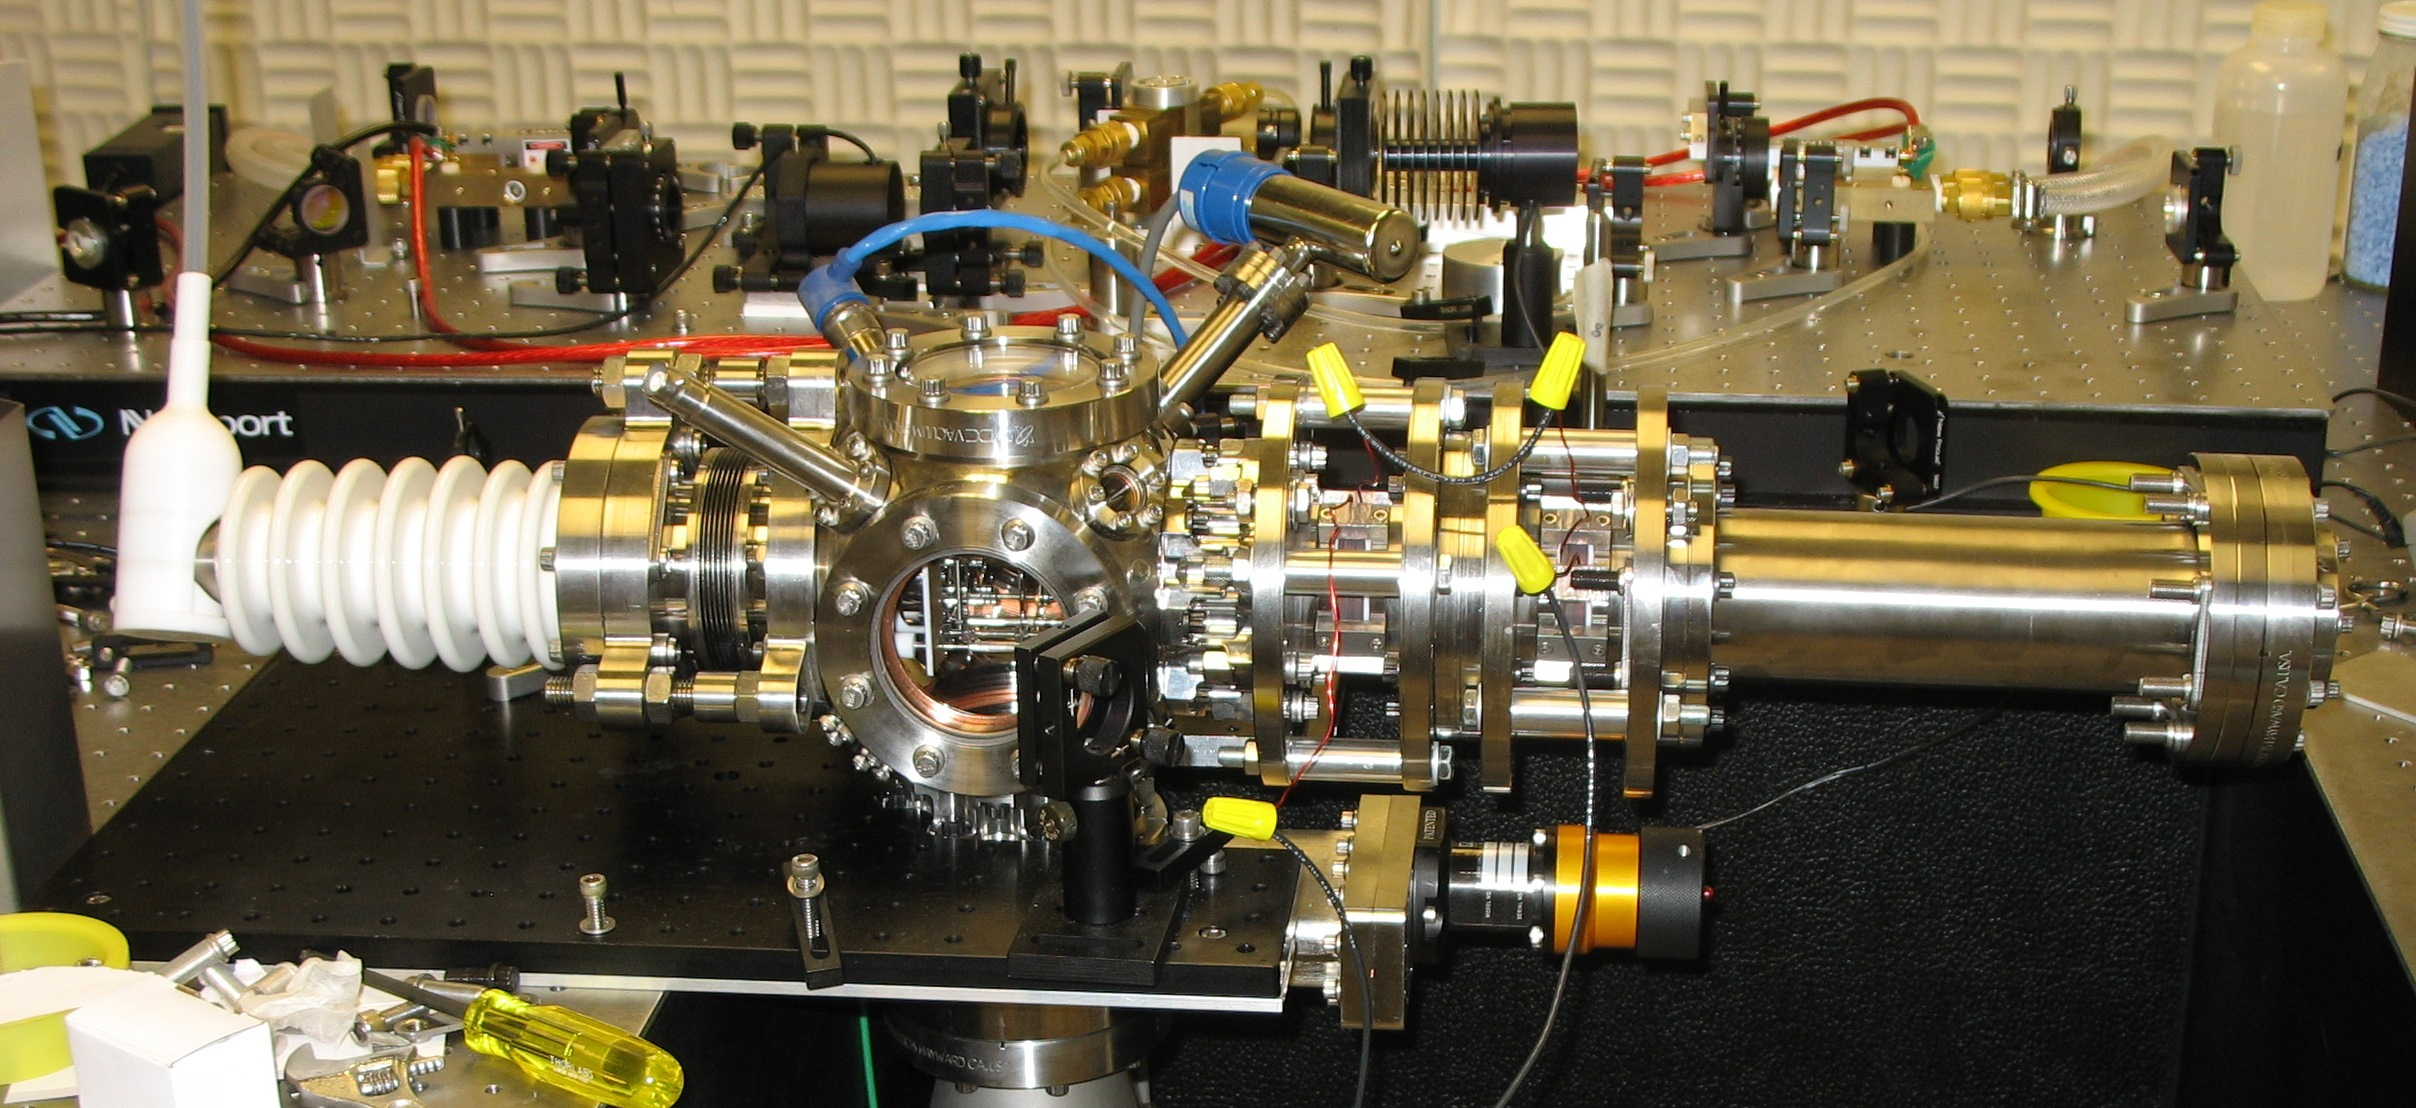
\includegraphics[width=0.9\linewidth]{column_lenses}};
      \end{pgfonlayer}
      \draw<2->
        [fill=orange] 
        (-2,-0.5)
        -- ++(0.2,0)
          node [midway,pin={below,fill=white:Photocathode}] {}
        -- ++(0,1)
          node [midway,inner sep=0.1] (source) {}
        -- ++(-0.2,0)
        -- cycle
      ;
      \draw<2->
        [fill=red]
        ($(source) + (2.35,0) $) node [inner sep=2mm] (lens1) {}
        arc (180:160:2)
        arc (20:-20:2)
          node (label lens1) {}
        arc (200:180:2)
      ;
      \draw<2->
        [fill=red]
        ($(source) + (3.4,0) $) node [inner sep=2mm] (lens2) {}
        arc (180:160:2)
        arc (20:-20:2)
          node (label lens2) {}
        arc (200:180:2)
      ;
      \node<2-> at ($(lens1)!0.5!(lens2) + (0,-1.5)$) (lens label) [red,fill=white] {Magnetic Lenses};
      \foreach \x in {1,2}
        \draw<2-> [white,thick] (lens label) -- (label lens\x);
      \draw<2-> 
        [fill=green!40]
        ($(source) + (6.5,0)$) node [inner sep=0] (detector) {}
          ellipse (0.2 and 0.5) 
            node at ($(source) + (6.5,-0.5)$) [pin={below,fill=white:Detector}] {}
      ;
      \draw<3->
        [green,very thick]
        (-5.2,-0.7)
        -- (-0.7,-0.7)
          node [pos=0.2,below=2mm,fill=white] {Laser}
        -- (source.east)
      ;
      \draw<5-> [fill=gray!60]
        ($(lens1)!0.5!(lens2) + (-0.05,0.5)$)
        node [pin={above,fill=white:{RF Cavity}}] {}
        rectangle ++(0.3,-1)
      ;
      \begin{pgfonlayer}{below-main}
        \fill<4->
          [blue!40]
          (source)
          -- (lens1.north)
          -- (lens2.north)
          -- (detector.east)
            node [midway,above=5mm,fill=white] {Electron Beam}
          -- (lens2.south)
          -- (lens1.south)
        ;
      \end{pgfonlayer}
    \end{tikzpicture}
  \end{figure}
  \visible<6->{And yes, we fixed the drooping column mount}
\end{frame}

\begin{frame}{Primary Laser Oscillator}
  Diode-pumped Thermal Lens Shaped (TLS) Yb:KGW primary laser:
  \begin{itemize}
    \item<2-> 250 fs pulse duration
    \item<3-> 2W output at 63MHz (31 nJ)
    \item<4-> Fundamental: 1047nm ($\hbar \omega$ = 1.2eV)
    \item<5-> 2$\hbar \omega = $ 2.47eV (524nm): $\Rightarrow$ Au plasmon, 2 photon over Ta
    \item<6-> 4$\hbar \omega = $ 4.75eV (262nm): $\Rightarrow$ 1 photon over Ta
    \item<7-> Adjustable laser cavity length allows matching:
    \begin{itemize}
      \item<7-> Laser repetition rate
      \item<7-> RF cavity resonance frequency
    \end{itemize}
  \end{itemize}
  \begin{figure}
    \centering
    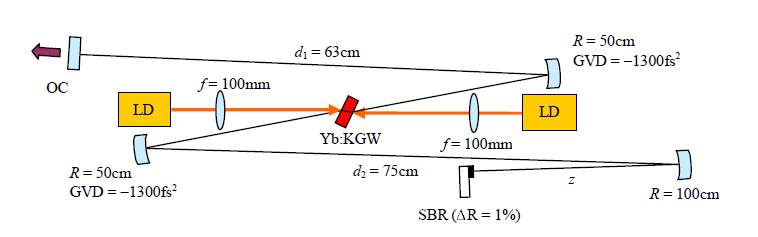
\includegraphics{laser_schematic}
  \end{figure}
\end{frame}

